\section{Preliminaries}\label{chap4-sec:background}
%In this section, we introduce the necessary background on \ldp~for graph analysis followed by .\\\\\noindent
\textbf{Notation.}
Throughout this paper, let $G = (V, E)$ be an undirected 
graph with $V$ and $E$ representing the set of nodes (vertices) and edges, respectively. We assume a graph with $n \in \mathbb{N}$ nodes, i.e., $V = [n]$ where $[n]$ denotes the set $\{1,2,\cdots,n\}$. Let $\calG$ denote the domain of all graphs with $n$ nodes. Each node $i \in V$ corresponds to a user $\DO_i$. Let $l_i \in \{0,1\}^n$ be the adjacency list for $\DO_i, i \in [n]$ where bit $l_i[j], j \in [n]$ encodes the edge $e_{ij}$ between a pair of users $\DO_i$ and $\DO_j$. Specifically, $l_i[j]=1$ if $e_{ij}\in E$ and $e_{ij}=0$ otherwise. %Note that $l_i$ is the $i$-th row of the adjacency matrix $L$ of the graph $G$. 
Let $\textbf{d}=\langle d_1, \ldots, d_n\rangle \in \R^n$ denote the vector of degrees in $G$. $m$ denotes the number of malicious users.


\subsection{Local Differential Privacy for Graphs}\label{chap4-sec:ldp}
%Differential privacy (\DP) is a quantifiable measure of the stability of the output of a randomized mechanism to changes to its input. 
Our paper focuses on the \textit{local} model of \DP, one of the most popular models. % There are two popular models of differential privacy, \textit{local} and \textit{central}.
The local model consists of a set of individual users (\DO) and an untrusted data aggregator (analyst); each user perturbs their data using a (local) \DP~algorithm and sends it to the aggregator which uses these noisy data to estimate certain statistics of the entire dataset. %Thus, the \ldp~model allows gleaning of useful information from the dataset without requiring the data owners to trust any third-party entity. %This makes it an attractive model for commercial deployment~\cite{Apple,Rappor1,Rappor2,Uber}.
  %An edge $e_{ij}$ is shared between two users $\DO_i$ and $\DO_j$. 
 
The most popular privacy guarantee for graphs in the local setting is known as \textit{edge \ldp}~\cite{Nissim_STOC07,Raskhodnikova_Encyclopedia16} which protects the existence of an edge between any two users. In other words, on observing the output, an adversary cannot distinguish between two graphs that differ in a single edge. Formally, we have:
\begin{defn}[$\epsilon$-Edge~\ldp\cite{qin2017generating}]
    Let $R: \{0,1\}^n\mapsto \mathcal{X}$ be a randomized algorithm that takes an adajcency list $l \in \{0,1\}^n$
as input. We say $R(\cdot)$ provides $\epsilon$-edge LDP if for any two
neighboring lists $l,l' \in \{0,1\}^
n$ that differ in one bit (i.e., one
edge) and any output $s \in \mathcal{X}$,
\begin{gather} \mathrm{Pr}
[R(l) = s]\leq e^{\epsilon}\mathrm{Pr}[R(l') = s]
\end{gather}
\end{defn}
 


\begin{comment}As noted above, the knowledge of an edge in a graph is shared between two users. Motivated by this observation, recent work~\cite{imola2021locally,imola_communication-efficient_2022} has introduced a new notion of \DP~called relationship \DP~that considers both the users' outputs and \textit{hides an edge in a graph during the entire computation}. Formally, we have:
\begin{defn}[$\epsilon$-relationship \DP]  For $i \in [n]$,
let $R_i: \{0,1\}^n\mapsto \calX$ be the local randomizer of user $\DO_i$ that takes their adjacency list $l_i$ as input.
We say $\langle R_1(\cdot),\cdots,R_n(\cdot)\rangle$ provides $\epsilon$-relationship \DP~if for any
two neighboring graphs $G,G' \in \calG$ that differ in one edge and
for any $S\subseteq \calX^n$,
\begin{multline*}
\Pr[(R_1(l_1),\cdots,R_n(l_n)) = S]
\leq e^{\epsilon} \Pr[(R_1(l'_1),\cdots,R_n(l'_n))=S], \end{multline*}
where $l_i$ (respectively, $l_i'$)
is the $i$-th row of the adjacency
matrix of graph $G$ (respectively, $G'$).\end{defn}

Relationship \DP~is closely connected to the notion of edge \ldp~which is one of the most popular privacy guarantee for graphs \cite{Nissim_STOC07,Raskhodnikova_Encyclopedia16} in the \ldp~setting. 
$\epsilon$-edge \ldp~protects the information about an edge $e_{ij}$ from the adjacency list $l_i$ of a \textit{single} user $\DO_i$. On the other hand, relationship \DP~consider the outputs from \textit{both} users $\DO_i$ and $\DO_j$ and hides the \textit{edge as a  whole}. Formally, if each of the local randomizers $R_i(\cdot), i \in [n]$ satisfy $\epsilon$-edge \ldp, then $\langle R_1(\cdot),\cdots,R_n(\cdot)\rangle$ satisfies $2\epsilon$-relationship \DP~\cite{Nissim_STOC07,Raskhodnikova_Encyclopedia16}. Next, we describe two common privacy mechanisms for degree estimation.
% For the rest of the paper, we consider $\epsilon$-relationship \DP~degree estimation algorithms.
\end{comment}


%Two adajacency lists are defined to neighboring lists if 
\noindent\textbf{Randomized Response.} Randomized Response ($RR_\rho(\cdot)$)~\cite{RR} releases a bit $b \in \{0,1\}$ by
flipping it with probability $\rho = \frac{1}{1+e^\epsilon}$. We extend the
mechanism to inputs in $\{0,1\}^n$ by flipping each bit independently with
probability $\rho$ (Alg.~\ref{chap4-alg:rr} in App. \ref{chap4-app:background}) which satisfies
 $\epsilon$-edge \DP. 
 
\noindent\textbf{Laplace Mechanism.} 
The Laplace mechanism(\RLap) is a standard algorithm to achieve \DP~\cite{Dwork}. For degree estimation, each user $\DO_i$ simply reports $\tilde{d}_i=d_i+\eta, \eta \sim Lap(\frac{1}{\epsilon})$ where $Lap(b)$ represents the Laplace distribution with scale parameter $b$. This mechanism satisfies $\epsilon$-edge \DP. 

Every protocol used in this paper is based on randomized response, the Laplace mechanism, or a composition thereof, and it is easy to show each one satisfies $\epsilon$-edge LDP.

\subsection{Protocol Setup}
\noindent\textbf{Problem Statement.}  
We consider single round,  non-interactive protocols in which each user $\DO_i, i \in [n]$ runs the local randomizer
$R_i : \{0,1\}^n \rightarrow \calX$ for some output space $\calX$ on their adjacency lists $l_i$ (Fig. \ref{chap4-fig:setting}). The data aggregator collects the noisy responses and applies a function 
$D : \calX^n \rightarrow (\mathbb{N} \cup \{\bottom\})^d$ to produce final degree estimates  $\hat{\textbf{d}}=\langle \hd_1, \ldots, \hd_n\rangle)$. Here, $\hd_i$ is the aggregator's estimate for $d_i$ for user $\DO_i$. Note that the aggregator is allowed to output a special symbol $\bottom$ for a user $\DO_i$ if they believe the estimate $\hat{d}_i$ to be invalid (i.e., $\DO_i$ is malicious).
    \\\\
\noindent\textbf{Threat Model.}
In the execution of a protocol $\calP$, a subset of users $\calM \in [n]$ may be malicious. The malicious users may return arbitrary output with the goal of carrying out a poisoning attack on  $\calP$. Let
$m=|\calM|$ denote the number of malicious users. We refer to 
$\calH = [n] \setminus \calM$ as the set of honest users.
We do not make any assumptions on how the malicious users are instantiated in practice -- they could correspond to either fake accounts created by the adversary or a set of real accounts which have been compromised or a combination of both. 

Based on the specifications of the practical implementation of the \ldp, there is an important distinction between the way in which the malicious users may carry out their poisoning attacks. We outline them as follows:

\squishlist
    \item \textbf{Input Poisoning.} In this threat model, the users do not have access to the implementation of the \ldp{} randomizer. For instance, mobile applications might run proprietary code which the users do not have permission to tamper with. Consequently, the only thing a malicious user can do is falsify their underlying input data, i.e.,  change their input from $l_i$ to an arbitrary $l_i'$, and then report $q_i = R_i(l_i')$ (Fig. \ref{chap4-fig:input}).
    
    \item \textbf{Response Poisoning.} This is a stronger threat model where a malicious user has direct control over the implementation of the \ldp{} randomizer. For instance, the user could hack into the mobile application collecting their data. Consequently, the user can completely bypass the randomizer and submit an arbitrary response $q_{i}$ (Fig. \ref{chap4-fig:response}) to the aggregator.
\squishend

Note that input poisoning attack applies to \textit{any} protocol, private or not, because a user is free to change their input anytime. However, response poisoning attacks are unique to \ldp{} -- the distinction between an user's input and their response is a characteristic of \ldp{} which we results in a separation in the efficacy of the two types of attacks (see Sec. \ref{chap4-sec:input-attacks} for details). 


\begin{figure}
    
    \centering
    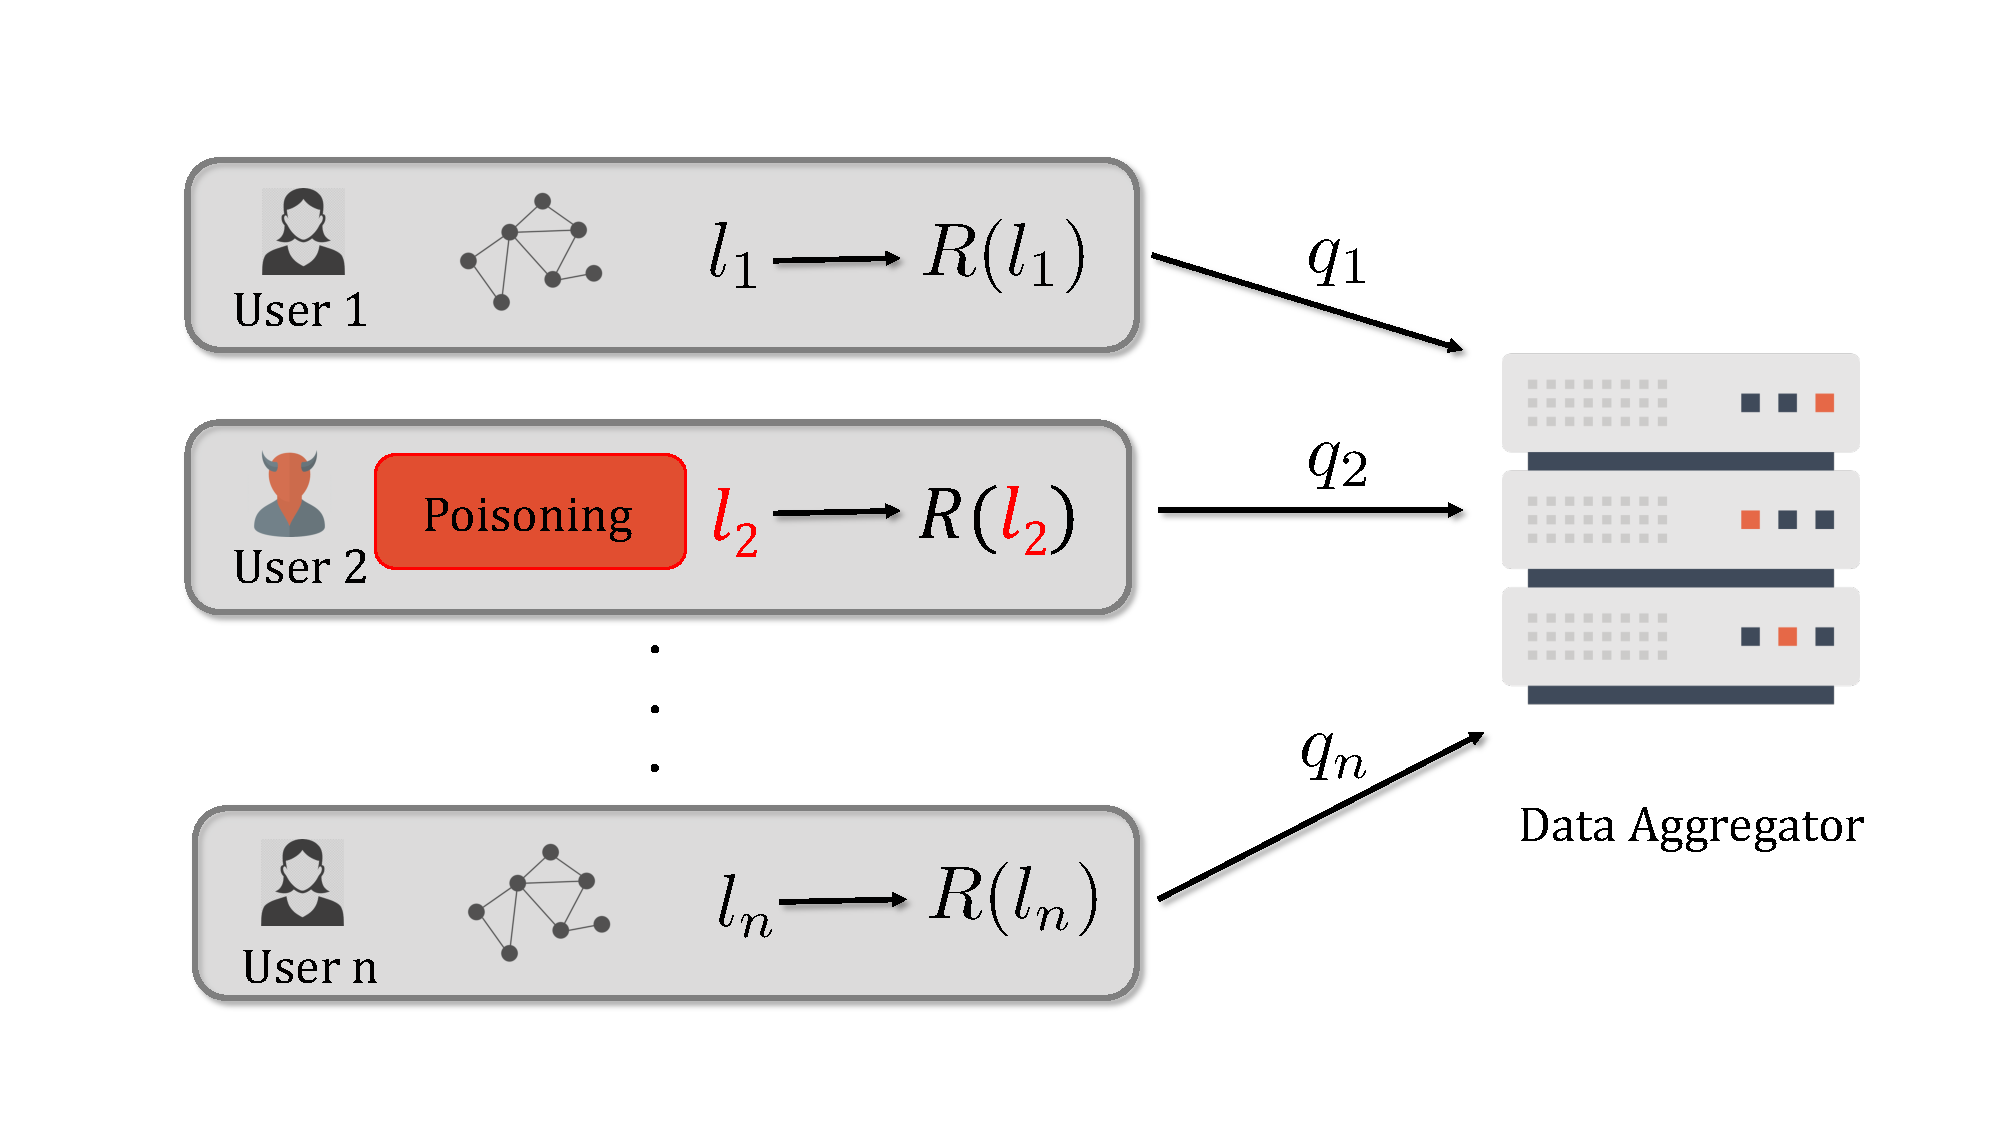
\includegraphics[width=0.8\columnwidth]{graph_pic_3.pdf}
    
    \caption{Input Poisoning Attack}
    \label{chap4-fig:input} 
        
\end{figure}
\begin{figure}[bt]
    \centering
 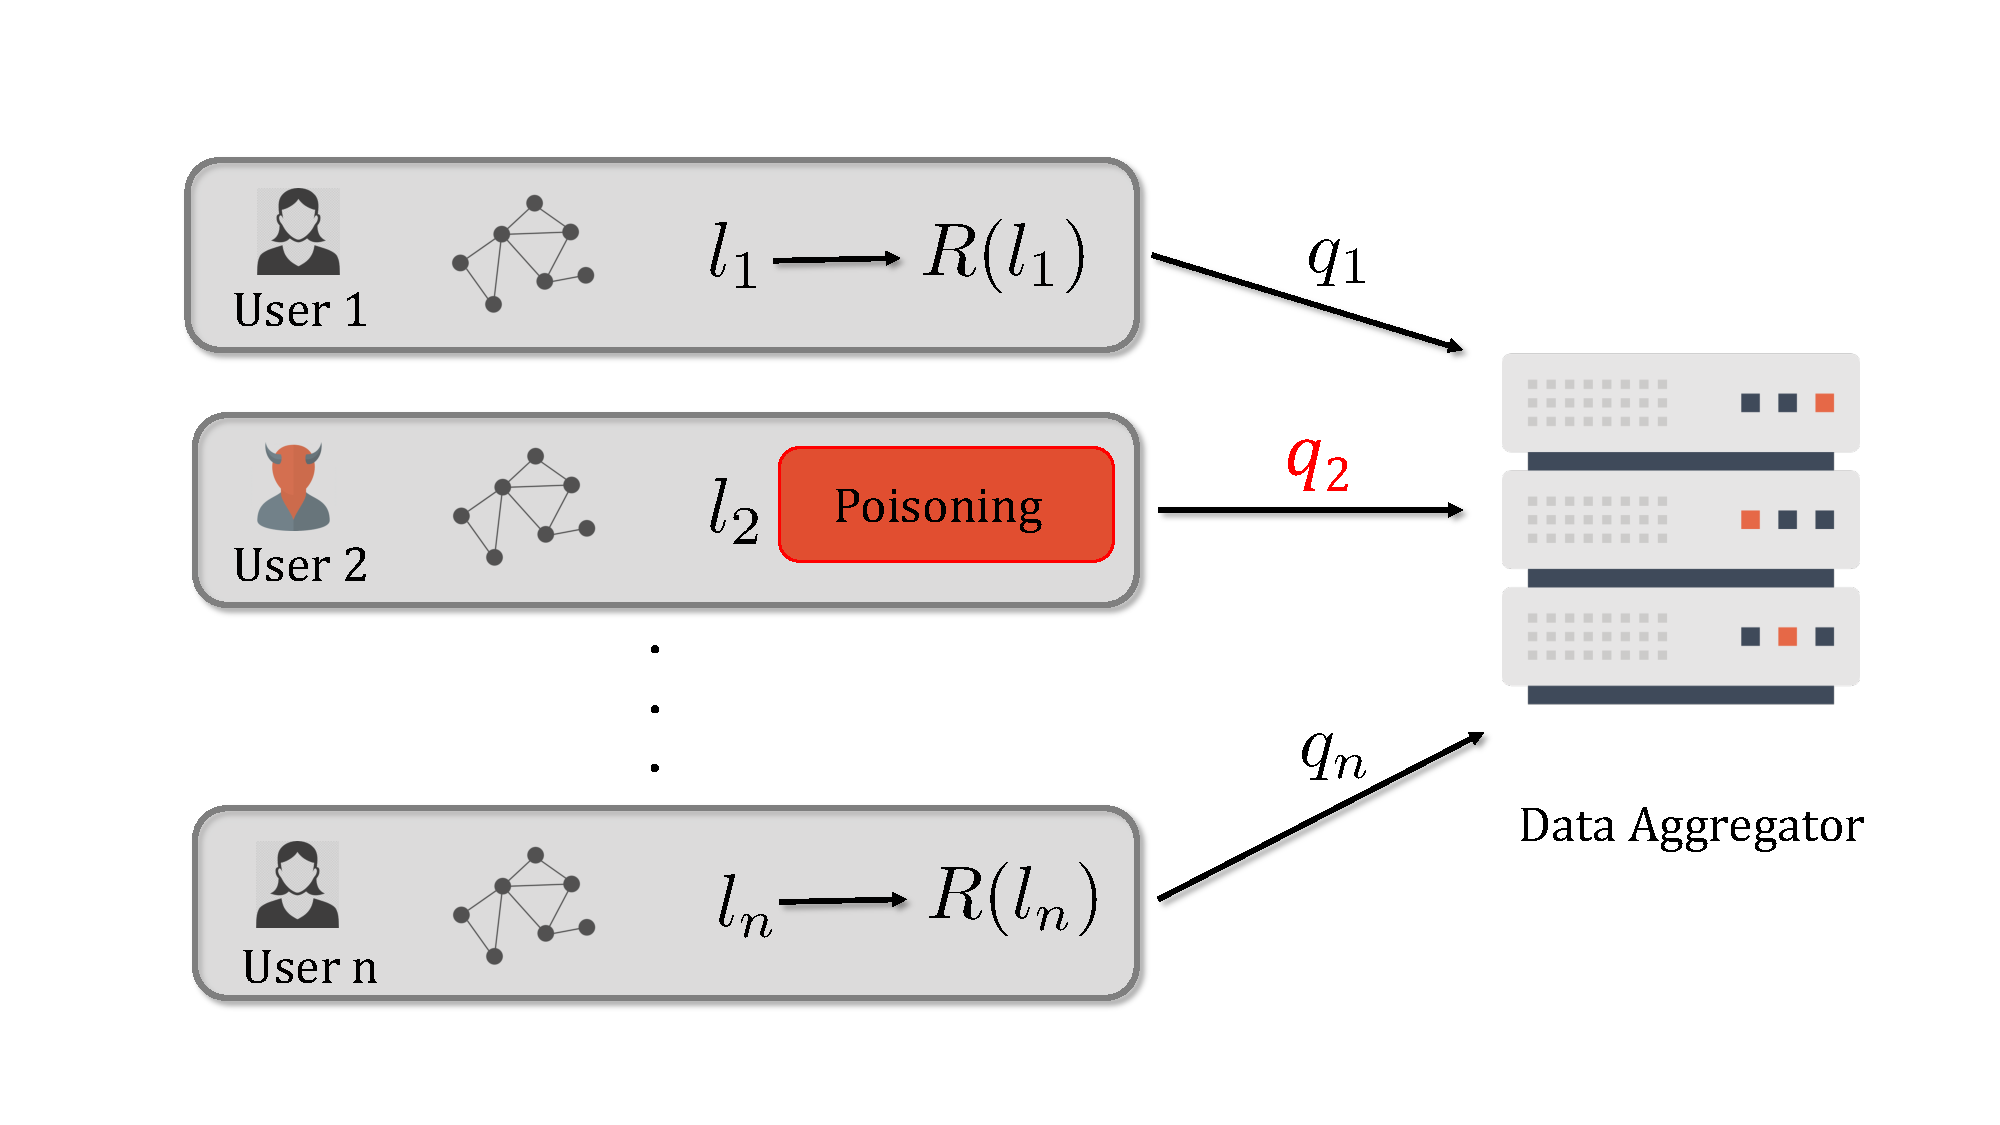
\includegraphics[width=0.8\columnwidth]{graph_pic_2.pdf}
     
   \caption{Response Poisoning Attack}
    \label{chap4-fig:response} 
\end{figure}





    \subsection{Motivating Attacks}\label{chap4-sec:attacks}

For the Laplace mechanism, \RLap, and randomized response mechanism, $RR_\rho$,  outlined in Sec.~\ref{chap4-sec:ldp}, we present two concrete motivating attacks. We consider the attacks in the context of the task of influential node identification, where the goal of the data aggregator is to identify certain nodes with a high measure of ``influence". This is useful for various applications where the influential nodes are selected for disseminating information/advertisement. Here, we consider the simplest measure of influence -- degree; nodes with the top-$k$ degrees are selected as the influencers. With the goal of modifying the influence of different users, a malicious user may choose to carry out the following attacks:
    \\\\\noindent\textbf{Degree Inflation Attack.} In this attack, a target malicious user $\DO_t$ wants to get themselves selected as an influential node. For \RLap, since each user sends their degree $d_i$ plus Laplace noise, the target user maximizes their degree estimate by simply sending $n-1$. 

For $RR_\rho$, the target malicious user $\DO_t$ colludes with a set of other users  (for instance, by injecting fake users) as follows. All the non-target malicious users $\DO_i, i \in \calM\setminus t$ report $1$ for the edges corresponding to $\DO_t$. Additionally, $\DO_t$ reports an all-one list.     \\\\
\noindent\textbf{Degree Deflation Attack.}   In this attack, the target is an honest user $\DO_t \in \calH$ who is being victimized by a set of malicious users (for instance, the adversary compromises a set of real accounts with an edge to $\DO_t$) -- $\calM$ wants to ensure that $\DO_t$ is \textit{not} selected as an influential node. The attack strategy is to decrease the aggregator's degree estimate $\hd_t$ for $\DO_t$. For \RLap, there is no way for the malicious party to influence $\hd_t$. However, for randomized response, the malicious users may report $0$ for each edge in $\calM$ connected to $\DO_t$, reducing their degree by this amount. %\ji{We might be able to improve degree deflation attacks!}
